\documentclass[10pt,a4paper]{article}
\usepackage[utf8]{inputenc}
\usepackage[francais]{babel}
\usepackage[T1]{fontenc}
\usepackage[left=2cm,right=2cm,top=2cm,bottom=2cm]{geometry}
\usepackage{graphicx}
\usepackage{moreverb}
\author{H4311}
\title{Document de Conception}

\begin{document}

\maketitle
\tableofcontents

\section{Introduction}
\subsection{Rappel du contexte}
Ce projet 4IF consiste en la conception et la réalisation d'un processeur XML comprenant les fonctionnalités suivantes : analyse syntaxique d'une DTD, analyse syntaxique d'un XML, analyse syntaxique d'un XSL, vérifications sémantiques d'un XML par rapport à une DTD donnée, transformation d'un XML par rapport à une feuille XSLT.

\subsection{Portée de ce document}
Ce document de conception présente les diagrammes de classes utilisés pour stocker en mémoire une arborescence XML et une feuille DTD, ainsi que les algorithmes de validation et de transformation.

\section{Modélisation}
\subsection{Feuille DTD}
Le schéma ci-dessous présente notre diagramme de classes au format UML pour le stockage d'une feuille DTD. Les méthodes n'ont pas été ajoutées afin de ne pas alourdir le diagramme et à la demande des enseignants.
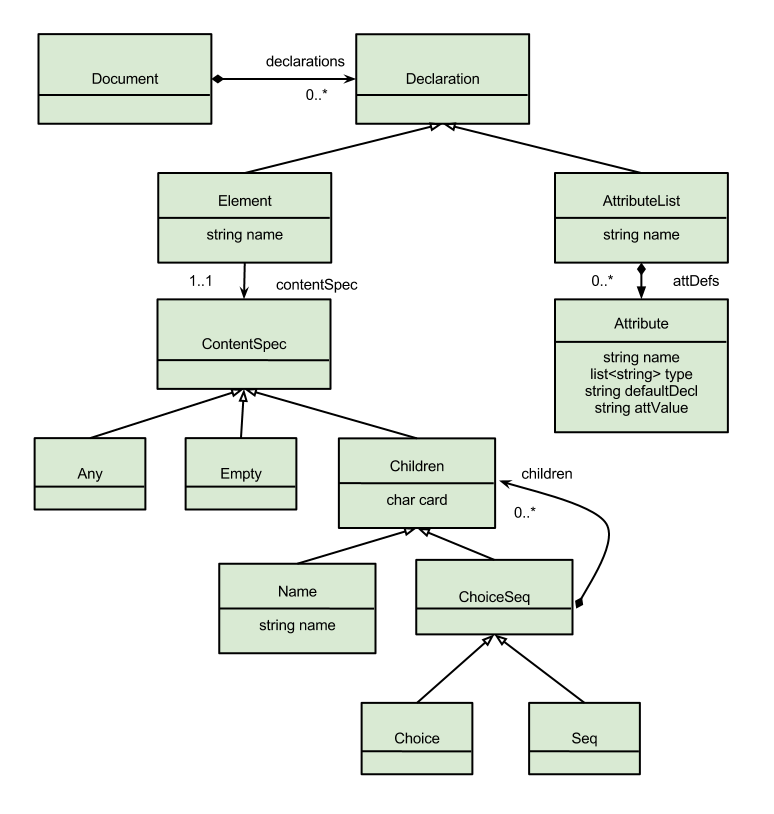
\includegraphics[scale=0.65]{DiagrammedeclasseDTD.png} 

\subsection{Document XML}
Le schéma ci-dessous présente notre diagramme de classes au format UML pour le stockage d'un document XML. Les méthodes n'ont pas été ajoutées afin de ne pas alourdir le diagramme et à la demande des enseignants.
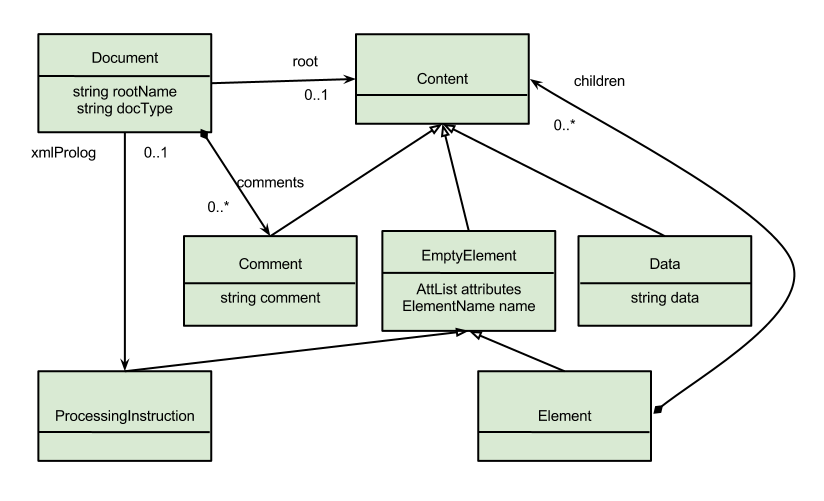
\includegraphics[scale=0.65]{DiagrammedeclasseXML.png} 

\section{Algorithmes}
\subsection{Validation}
Cet algorithme consiste en la validation d'un document XML par rapport à une DTD donnée, i.e en sa vérification sémantique.

\begin{description}
\item[Entrée :] un document XML bien formé et une feuille DTD bien formée.
\item[Sortie :] vrai si le document XML est conforme à la feuille, faux sinon.

En outre, des messages d'erreurs s'affichent sur la sortie d'erreur standard, permettant de diagnostiquer l'origine de l'erreur.
\end{description}

\paragraph{L'idée derrière l'algorithme :}
Nous partons d'un constat simple : les déclarations de contenus DTD ressemblent fortement à des expressions régulières (regex). Le principe de l'algorithme est donc le suivant :
\begin{itemize}
\item Pour chaque contenu XML, générer la chaine correspondant à ce que ce contenu a pour noeuds fils.
\item Pour chaque règle DTD, générer la regexp correspondant à cette règle.
\item Comparer la chaîne de contenu avec la règle DTD correspondante au nom de l'attribut.
\end{itemize}

\paragraph{Regex créées par les éléments dtd}
Ces fonctions servent à créer les regex des différents éléments dtd qui servent à la validation par la suite. Tous les enfants de dtd::Children dans la hiérarchie de classes dtd possèdent une version différente. Les premières méthodes ne prennent pas d'arguments et renvoient une chaîne correspondant à la regex générée. Les deux dernières méthodes renseignent la méthode template dtd:ChoiceSeq:regex.

\begin{itemize}
\item[dtd:Name:regex] :
\begin{verbatimtab}
	chaine regex := "(" + name + ",)"
	Si card est défini, alors
		regex += card
	FinSi
	Renvoyer regex
\end{verbatimtab}
\item[dtd:ChoiceSeq:regex] :
\begin{verbatimtab}
	caractère regexSep = getRegexSep()
	chaine regex := "("
	regex += children.premierElement.regex
	Pour tous les autres éléments c de la liste children,
		Si regexSep est non nul, alors
			regex += regexSep
		FinSi
		regex += c.regex
	FinPour
	regex += ")"
	Si card est non nul, alors
		regex += card
	FinSi
	retourner regex
\end{verbatimtab}
\item[dtd:Any:regex] :
\begin{verbatim}
	retourner ".*"
\end{verbatim}
\item[dtd:Empty:regex] :
\begin{verbatim}
	retourner ""
\end{verbatim}
\item[dtd:Choice:getRegexSep] :
\begin{verbatim}
	retourner '|'
\end{verbatim}
\item[dtd:Seq:getRegexSep] :
\begin{verbatim}
	retourner vide
\end{verbatim}
\end{itemize}

\paragraph{Validation d'un élément}
\begin{description}
\item[Spécification :] Valide un noeud de l’arbre XML conformément à la DTD.
\item[Paramètres :]
\begin{itemize}
\item[content] : contenu correspondant au noeud courant.
\item[elements] : liste des éléments définis par la dtd.
\item[attributeList] : liste de liste d’attributs définis par la dtd
\end{itemize}
\item[Retour :] vrai si le noeud a été correctement validé, faux sinon.
\end{description}

\begin{verbatimtab}
validationNode(Content content, liste Element elements, list AttributeList attributeList) : booléen
Début
Si elem := content, est de type Element alors
	chaine nomBalise := elem.nom
	// Valider les attributs
	// On récupère la liste des attributs de la dtd
	Pour chaque liste d'attributs listeAtt de attributeList, faire
		Si listeAtt.nom == nomBalise, alors
			sortir de la boucle
		FinSi
	FinPour	
	Si on est sortis de la boucle manuellement,
		attributs := listeAtt.attributs
	FinSi
	// On parcourt la liste des attributs xml pour les valider
	attributsElem := elem.attributsListe
	Si taille(attributsElem) > 0, alors
		Pour tous les xml de attributsElem, faire
			booléen trouvé := faux
			Pour tous les attributs att de attributs, faire
				Si xml == att, alors
					trouvé := vrai
					sortir de la boucle
				FinSi
			FinPour
			Si trouvé == faux, alors
				Erreur := "Attribut non trouvé"
				Renvoyer FAUX
			FinSi
		FinPour
	FinSi
		
	Chaine regex = chaine vide
	Pour tous les éléments e de elements, faire
		Si e.nom == nomBalise, alors
			regex = e.nom
		FinSi
	FinPour
		
	Si regex est vide, alors
		Renvoyer faux
	FinSi
		
	children := elem.enfants
	Chaine chaineChildren = chaine vide
	Pour chaque c de children, faire
		Si c est de type Element ou EmptyElement, alors
			chaineChildren += c.nom + ','
		Sinon
			Si c est de type Data, alors
				chaineChildren += "#PCDATA,"
			FinSi
		FinSi
	FinPour

	Si la chaîne chaineChildren ne valide pas l'expression régulière regex, alors
		Renvoyer faux
    	Sinon
    		Pour chaque c de children, faire
    			resultat := Appeler récursivement validationNode(c, elements, attributesList)
    			Si resultat est faux,
    				Renvoyer faux
    			FinSi
    		FinPour
    	FinSi
    	
    	Renvoyer vrai
Fin
\end{verbatimtab}

\paragraph{Validation du document}
\begin{description}
\item[Spécification :] Valide un arbre XML par rapport à une structure de DTD.
\item[Paramètres :]
\begin{itemize}
\item[dtd] : feuille DTD.
\item[xml] : document XML.
\end{itemize}
\item[Retour :] vrai si le document a été correctement validé, faux sinon.
\end{description}

\begin{verbatimtab}
validationDocument(dtd::Document dtd, xml::Document xml) : booléen
Début
	Liste<dtd::Element> elements
	Liste<AttributesList> attributesList   
	Liste<Declarations> declarations := dtd.declarations
	
	Pour tous les d de declarations faire
		Si d est de type dtd::Element, alors
			Ajouter d à la suite de elements
		Sinon
       		Si d est de type dtd::AttributeList, alors
       			Ajouter att à la suite de attributesList
			Sinon
       			Erreur := "Une déclaration de la DTD n'est ni un dtd::Element 
       				ni un dtd::Attribute"
		FinSi
	FinPour
   
	Retourner validationNode(xml.elementRacine, elements, attributesList);
Fin
\end{verbatimtab}

\subsection{Analyse et validation XSL}
Le schéma ci-dessous résume le fonctionnement de l'algorithme :

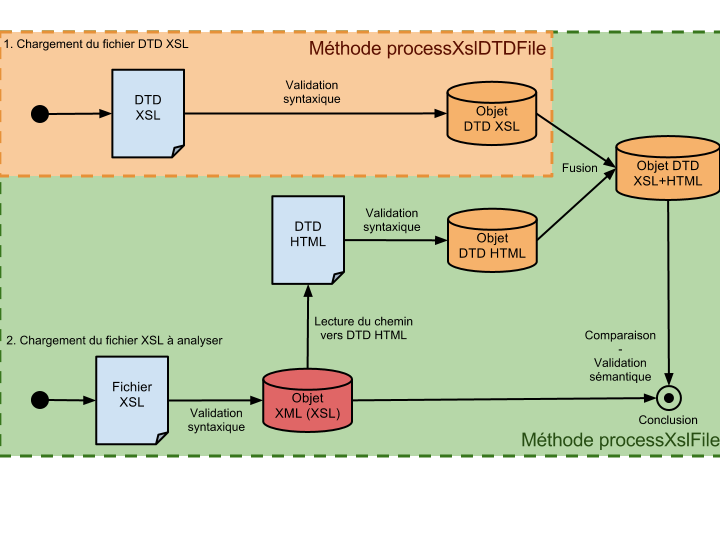
\includegraphics[scale=0.65]{Algorithmes.png}
\subsection{Génération XSL}
\subsubsection{Méthode de traitement du document XSL}
\begin{description}
\item[Spécification :] Valide, à l’aide notamment de la DTD XSL précédemment fournie, et génère la structure du XSL fournie, puis le sauvegarde (si valide) en attribut de cet objet XSLProcessor.

Le chemin vers la DTD HTML à employer pour valider ces éléments dans le XSL doit se trouver en valeur de l’attribut "xmlns:xsl" de l’élement "xsl:stylesheet" situé sous la racine du XSL. Cette DTD fera également l’objet d’une vérification syntaxique (arrêt du traitement si invalide).

Si le document XSL est invalide, l’ancienne valeur de l’attribut sera conservée.

\item[Paramètres] :
\begin{itemize}
\item[xml:Document newXslDoc] Document XSL (validé et généré).
\end{itemize}

\item[Retour] : Vrai si le XSL est valide et a été sauvé en mémoire, faux sinon.
\end{description}

\begin{verbatimtab}
processXslFile(xml:Document newXsldoc) : booléen
Début
	Si pas de DTD XSL fournie précédemment, alors
		Retourner faux;
	FinSi
	
	// Recherche de la DTD HTML employée par ce XSL.
	// Le chemin vers ce fichier se trouve dans l’attribut "xmlns:xsl" 
	// de l’élement "xsl:stylesheet" :
	Liste<Content> enfantsRootXSL := newXslDoc.rootElement.children
	EmptyElement elStylesheet := Null
	Pour chaque Content el dans enfantsRootXSL, faire :
		Si el de type Element et el.nom == “xsl:stylesheet", alors :
			elStylesheet := el
			sortir de la boucle
		FinSi
	FinPour
    
	Si elStylesheet nul, alors :
		Retourner faux // Elément contenant le lien vers la DTD HTML non-trouvé.
	FinSi
    
	Chaine attrXMLNS := elStylesheet.valeurAttribut("xmlns:xsl")
	Si attrXMLNS vide, alors :
		Retourner faux // Attribut "xmlns:xsl" vide ou inexistant.
	FinSi
	
	// Ouverture et validation syntaxique de la DTD HTML :
	Document htmlDTDdoc := parseXML(attrXMLNS);
	Si htmlDTDdoc nul, alors
		Retourner faux; // Erreur syntaxique dans la DTD HTML.
	Sinon Si htmlDTDdoc a une racine vide ou invalide, alors
		Retourner faux; // Erreur de structure dans la DTD HTML.
	FinSi
	
	// Fusion des deux DTD, XSL et HTML, pour obtenir la DTD totale à appliquer pour ce document
	// XSL : 
	// Pour cela, on copie dans la DTD HTML (temporaire, valable que pour ce document 
	// XSL) les déclarations de la DTD XSL (mémorisée, valable pour de multiples documents XSL).
	// On validera ce document avec la DTD HTML ainsi étendue.
	// De plus, pour ne pas supprimer les déclarations XSL à la suppression de la DTD HTML, 
	// nous copions dans un premier temps la liste des déclarations HTML, 
	// que nous restaurerons avant la suppression, afin que celle-ci n’affecte que les
	// déclarations HTML et pas XSL.
	Liste<Content> htmlElements := copie de htmlDTDdoc.rootElement.children
	htmlDTDdoc.rootElement.children += xslhtmlDTDdoc->rootElement.children // fusion
	
	// Analyse sémantique du XSL à partir de cette DTD :
	bool semanticCorrectness :=  DTDValidator.validate(newXsldoc, xslhtmlDTDdoc)
	Si semanticCorrectness faux, alors
		Supprimer htmlDTDdoc
		Retourner faux // XSL sémantiquement invalide.
	FinSi

	// Tout est OK. On met à jour l’attribut xslDoc de l’objet :
	Supprimer xslDoc
	xslDoc := newXsldoc
	Supprimer htmlDTDdoc;

	Retourner vrai
Fin
\end{verbatimtab}

\subsubsection{Génération du HTML à partir d’un document XML et d’une fiche XSL}
\paragraph{Méthode publique de génération}
\begin{description}
\item[Spécification :] Valide, à l’aide notamment d’une DTD XML, le document, puis génère à partir de la feuille XSL précédemment validée le document HTML correspondant.
\item[Paramètres :] 
\begin{itemize}
\item[xmlDoc] : Document XML (validé et traité).
\end{itemize}
\item[Retour :] Le document HTML généré, ou NULL si erreur.
\end{description}

\begin{verbatimtab}
generateHtmlFile(xml:Document xmlDoc), retourne xml:Document
Début
	Element XSLnode := findTemplate(xmlDoc.rootElement)
	Liste<Element> listElementsHTML := generateHTML(XSLnodeChild, xmlDoc.rootElement)
	Element racineHTML = Null
	Si taille(listElementsHTML) > 1, alors :
	// XSL n'ayant pas généré de racine, on en ajoute une
		racineHTML := nouvel Element(), de nom "null", pour lequel l'ensemble des éléments
			enfants sera constitué de la liste listElementsHTML
	Sinon Si taille(listElementsHTML) == 1, alors :
		racineHTML := listElementsHTML[0]
	FinSi
   
	Document docHTML := nouveau Document()
	docHTML.setRootElement(racineHTML)
	Retourner docHTML;
Fin
\end{verbatimtab}

\paragraph{Méthode privée de génération récursive}
\begin{description}
\item[Spécification] Applique récursivement les templates XSL aux noeuds XML, et retourne les éléments HTML ainsi générés.

Si aucun template n’est donné en paramètre (NULL), les données internes du noeud XML courant seront ajoutées sans modifications dans le HTML, et les éléments XDML fils seront traités récursivement (d’après la norme).
\item[Paramètres]
\begin{itemize}
\item[XSLNode] Template XSL à appliquer.
\item[XMLNode] Noeud XML à parcourir.
\item[htmlNode] Noeud HTML en cours de génération (utilisé pour xsl::attribute).
\end{itemize}
\item[Retour] Liste des éléments HTML générés.
\end{description}

\begin{verbatimtab}
generateHtmlElement(Element xslNode, Content xmlNode, Element htmlNode), retourne Liste<Content>
Début
	Liste<Content> htmlNodeChildren
	Si xslNode != NULL, alors // On applique le template fourni
		Pour chaque enfant itXSL de xslNode, faire :
			Content htmlChild
			Si itXSL de type EmptyElement ou Element, alors
				Si itXSL élément HTML, alors :  // On le copie comme tel, en 
				// parcourant ses enfants s’il en a :
					Conversion de itXSL en Element.
					htmlChild.setName(itXSL.nom)
					htmlChild.setAttList(itXSL.getAttList())
					htmlChild.appendChildren(generateHtmlElement
						(itXSL, xmlNode, htmlChild))
					htmlNodeChildren.ajouter(htmlChild)
				Sinon Si itXSL.nom == "apply-templates", alors :
				// Pour chaque enfant du noeud XML, on tente d’appliquer 
				// un nouveau template :
					Pour chaque enfant-élément itXML de xmlNode, faire :
						xslNodeChild := findTemplate(itXML.nom)
						list<Content> applyChildren :=
						generateHtmlElement(xslNodeChild, itXML, htmlChild)
						htmlNodeChildren.ajouter(applyChildren)
					FinPour
				Sinon Si itXSLEmp.nom == "value-of", alors :
					// On récupère la valeur demandée via XPath :
					Chaine select := xmlNode.getAttributeValue("select")
					Chaine xPathResult := xpath::find(xmlNode, select)
					// On crée la “Data” contenant cette valeur :

					htmlChild := new Data(xPathResult)
					htmlNodeChildren.ajouter(htmlChild);
				Sinon Si itXSLEmp.nom == "attribute", alors :
					// On génère la valeur Data de cet élément XSL, à donner 
					// à l’attribut HTML :
					Chaine data := generateHtmlElement(itXSLEle, xmlNode, htmlNode)
					// Création de l’attribut du noeud HTML courant, avec 
					// cette valeur :
					htmlNode.addAttribute(itXSL.getAttributeValue("name"), data);
				FinSi                   
			Sinon, faire : // L’enfant XSL est de type Data :
				htmlChild := new Data(itXSLDat.getData());
				htmlNodeChildren.ajouter(htmlChild);
			FinSi
		FinPour
	Sinon, faire : // Si aucun template n’est donné, on ne fait que copier dans le HTML les 
	// enfants Data du noeud XML, et tenter d’appliquer des templates 
	// aux autres enfants
		Pour chaque enfant itXML de xmlNode, faire :
			Si itXML de type Data, alors :
				htmlNodeChildren.ajouter(itXMLDat);
			Sinon, faire :
				Element xslNodeChild := findTemplate(itXML.nom) // On cherche un 
				// template à appliquer à cet enfant-noeud.
				Liste<Content> contentChildren := generateHtmlElement
					(xslNodeChild, itXML, htmlNode) 
				// On génère récursivement le HTML pour cet enfant.
			FinSi
		FinPour
	FinSi
	Retourne htmlNodeChildren;
Fin
\end{verbatimtab}

\paragraph{Méthode privée de recherche de template}
\begin{description}
\item[Spécification :] Recherche dans le XSL le template dont la valeur de l’attribut “match” correspond au nom donné.
\item[Paramètres :]
\begin{itemize}
\item[XSLnode] Template XSL à appliquer.
\item[XMLnode] Noeud XML à parcourir.
\end{itemize}
\item[Retour] Liste des éléments HTML générés.
\end{description}

\begin{verbatimtab}
findTemplate( string nom ), retourne Element
Début
    Pour chaque noeud sous la racine de la feuille XSL, faire :
        Si noeud de type Element et noeud.nom == "template" et 
        noeud.GetAttributeValue("match") == nom, alors :
            Retourner noeud
        FinSi
    FinPour
    Retourner NULL;
Fin
\end{verbatimtab}


\end{document}